\documentclass[11pt, a4paper]{article}

% 导入常用的宏包
\usepackage[utf8]{inputenc} % 编码设置
\usepackage[
    a4paper,
    left=2.5cm,
    right=2.5cm,
    top=2cm,
    bottom=2cm
]{geometry}

\usepackage{amsmath} % 支持数学环境中的 \text 命令
\usepackage{graphicx} % 插入图片
\usepackage{booktabs} % 制作专业的三线表
\usepackage{hyperref} % 添加目录和引用的超链接
\usepackage{float} % 控制图表浮动位置
\usepackage{cite} % 参考文献引用
\usepackage{titlesec} % 自定义标题格式
\usepackage{setspace} % 行距设置
\usepackage{pdflscape}

\usepackage[style=ieee]{biblatex}
\addbibresource{reference.bib}

% 处理段落缩进与间距
\usepackage{parskip} % 全局取消首行缩进，并在段落之间自动增加适宜的空白间距

\setstretch{1.15} % 设置1.15倍行距

% 报告标题与作者信息
\title{\textbf{HAPSeat: Design and Implementation of a Multimodal Posture Support Cushion}}
\author{
\textbf{Group 3} \\
Crist Lian, Yange Sun, Junmou Tang, Shiyue Yang, Lechen Zha
}
%%%%%%%%%%%%%% 【日期】 %%%%%%%%%%%%%%%%%
\date{March 27, 2026}

\begin{document}

\maketitle
\thispagestyle{empty} % 首页不显示页码

\vspace*{\fill} 

% 摘要（居于页面中间部分）
\begin{abstract}
    \noindent This report presents HAPSeat, a seat cushion designed to detect unhealthy sitting patterns and support posture correction during prolonged seated work. The system combines eight force-sensitive resistors (FSRs) to monitor seat-pressure distribution with multimodal feedback consisting of a real-time visual heatmap interface and vibrotactile prompting. The design is based on four functional sitting indicators: left--right symmetry, anterior load sharing, reduced posterior collapse, and temporal postural variation. A proof-of-concept prototype integrating hardware, structural, and software subsystems was developed using an Arduino-based sensing and actuation architecture, a segmented 3D-printed baseplate, and threshold-based posture-detection logic. Preliminary prototype evaluation with approximately 30 users showed that the visual heatmap provided clear and intuitive feedback, while major posture changes such as forward, backward, left, and right leaning could be detected reliably once users were seated correctly. Although the vibration feedback was generally perceivable, its directional guidance effect remained limited, meaning that the current prototype functioned more effectively as a pressure-monitoring and posture-awareness system than as a fully developed haptic-guidance device. These findings demonstrate the feasibility of the overall system architecture while identifying actuation clarity, sensing resolution, and user adaptability as key priorities for future development.

    
    \vspace{0.5cm}
    %%%%%%%%%%%%%% 【字数】 %%%%%%%%%%%%%%%%%
    \begin{center}
        \textbf{Word Count: 2500}
    \end{center}
\end{abstract}

\vspace*{\fill} 


\newpage
\pagenumbering{arabic} % 从第二页开始显示阿拉伯数字页码

% 1. intro/idea/problem def-----------------------------
\section{Introduction and Problem Definition}

HAPSeat is a pressure-aware seat cushion designed to support posture correction through multimodal feedback. Its clinical relevance stems from the high burden of low back pain (LBP), which the World Health Organization identifies as the leading cause of disability worldwide; an estimated 619 million people were living with LBP in 2020, and this number is expected to increase further by 2050 \cite{WHO_LBP}. In office environments, this burden is aggravated by prolonged sitting and by persistent ergonomic deficiencies at the workstation level. Although the literature does not provide a single universal prevalence for "non-ergonomic chairs," observational studies consistently report substantial seating-related problems, including inadequate lumbar support and elevated ergonomic risk levels \cite{Sonne2012ROSA, Shahwan2021, Mohammadian2025}. These findings justify the need for seat-based interventions that act directly at the user--chair interface.

The design premise of HAPSeat is that unhealthy sitting is reflected not only in visible posture, but also in how load is distributed across the seat over time. Clinical seating guidance indicates that upright sitting should centre body weight over the ischial tuberosities, with pressure distributed as symmetrically as possible between the two sides \cite{QueenslandSeating}. Consistent with this, Akkarakittichoke and Janwantanakul found that office workers with chronic LBP showed more asymmetrical seat-pressure characteristics and fewer postural shifts during prolonged sitting \cite{Akkarakittichoke2017}. HAPSeat therefore uses force-sensitive resistors (FSRs) to detect pressure patterns associated with asymmetric or prolonged maladaptive sitting. When such a pattern is detected, the system provides feedback through two channels: a real-time visual interface showing seat-pressure distribution and vibrotactile feedback intended to guide, rather than repeatedly warn, the user. This concept is supported by haptics research showing that apparent tactile motion and related tactile illusions can communicate directional information through sparse actuator arrays, offering a potential low-attention feedback channel \cite{Israr2011TactileBrush, Israr2011ControlSpace, Pascher2023HaptiX}. HAPSeat is therefore conceived as a pressure-aware guidance device that combines intuitive visual monitoring with low-attention vibrotactile prompting.


% 2. 工作原理-----------------------------
\section{System Working Principle}

\subsection{Defining a Desirable Sitting State}
A desirable sitting state should be defined functionally rather than as one fixed “correct” posture. Current literature increasingly recognises that healthy sitting is dynamic and person-dependent rather than a rigid upright position maintained continuously \cite{Slater2019SitUpStraight}. For HAPSeat, a favourable pressure state is one in which load is relatively balanced between the left and right ischial tuberosities, some support is shared by the posterior thighs, excessive posterior drift toward the sacro-coccygeal region is avoided, and the user does not remain static for prolonged periods. This definition is consistent with clinical seating guidance and with evidence that workers with chronic low back pain exhibit more asymmetrical pressure patterns and fewer postural shifts during prolonged sitting \cite{QueenslandSeating, QSCIS_Skin, QSCIS_Ischial, Akkarakittichoke2017}. Accordingly, HAPSeat evaluates sitting using four practical indicators: left-right symmetry, thigh load sharing, antero-posterior pressure distribution, and temporal variation.

\begin{figure}[H] 
    \centering
    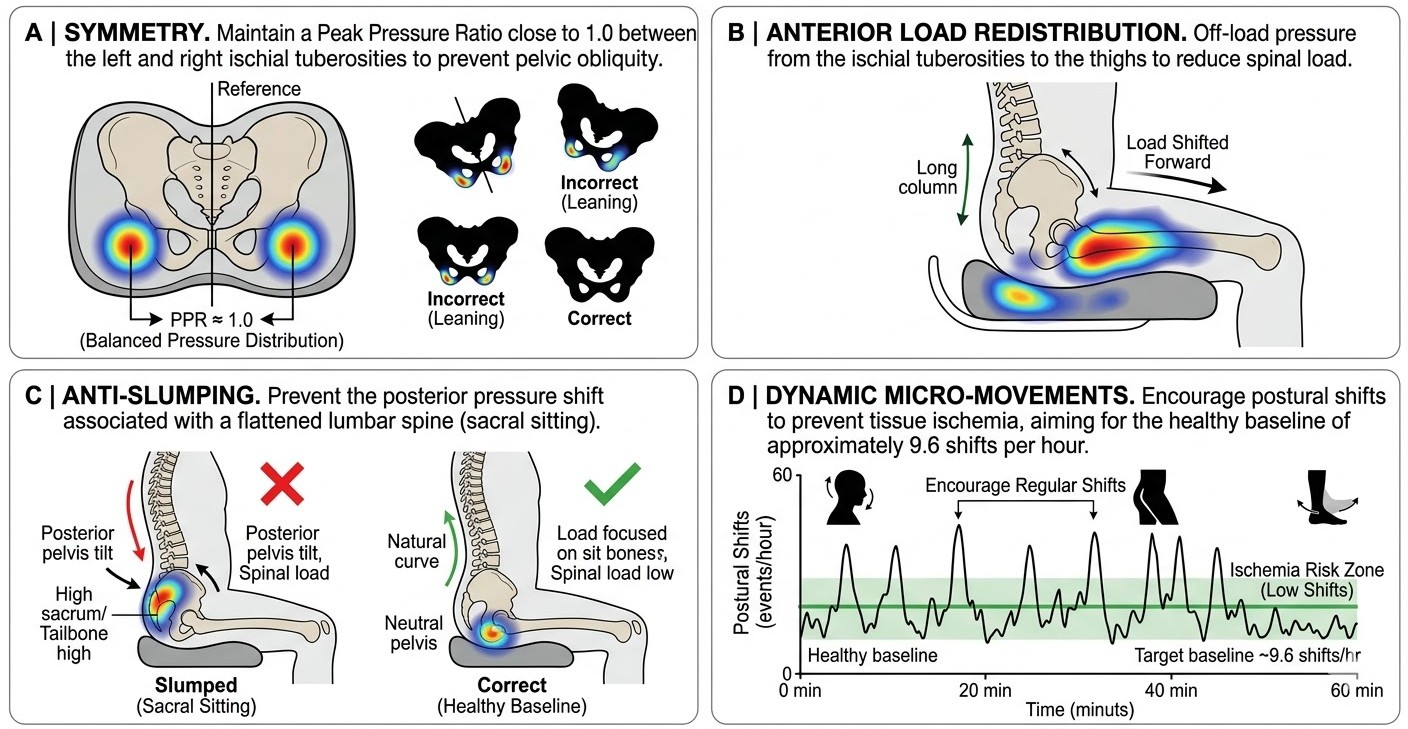
\includegraphics[width=1\linewidth]{2.jpg} 
    \caption{Visualisation of the four key healthy sitting biomechanical and haptic guidance goals.}
    \label{fig:biomechanical_goals}
\end{figure}

\subsection{Directional Haptic Guidance Through Tactile Illusion}

The feedback strategy of HAPSeat is based on directional vibrotactile guidance rather than simple warning vibration. In haptics research, apparent tactile motion and related phantom sensations show that sequential activation of spatially separated actuators can create a percept of movement across the skin. The \textit{Tactile Brush} framework demonstrated that sparse vibrotactile arrays can generate smooth directional cues through appropriate control of timing and intensity, while later studies confirmed that the resulting percept depends on stimulus onset timing, duration, body site, and actuator characteristics \cite{Israr2011TactileBrush, Israr2011ControlSpace}. For HAPSeat, this means that posture correction cues do not require dense actuator coverage. Instead, a limited number of motors can be activated in sequence to generate a directional sensation that encourages voluntary posture adjustment. This approach is especially suitable for seated work because vibrotactile cues can provide guidance without competing with visual attention and without relying on repetitive alarm-like reminders \cite{Pascher2023HaptiX, Brewster2004Tactons, Bark2015Vibrotactile}.

In the current prototype, this vibrotactile channel is complemented by a real-time visual heatmap interface, which provides a clearer and more reliable representation of pressure distribution during testing and demonstration.

\begin{figure}[H] 
    \centering
    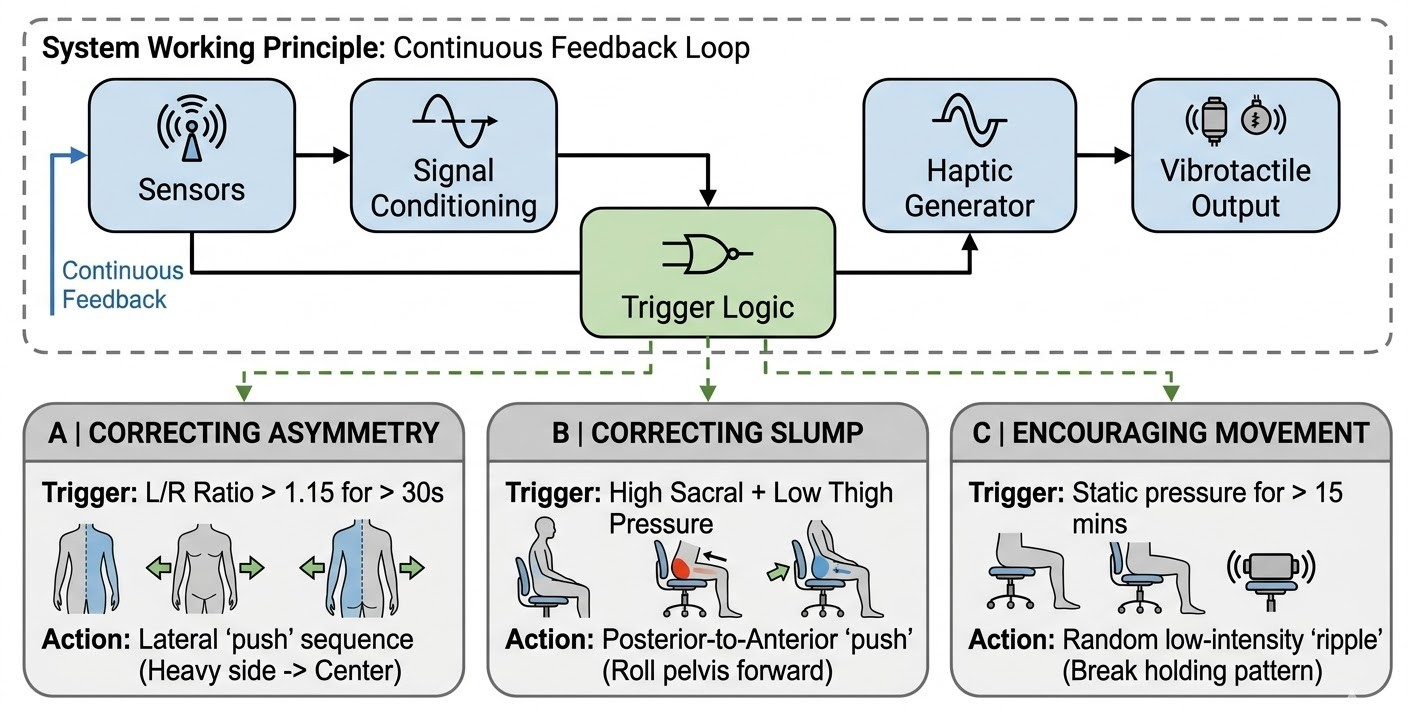
\includegraphics[width=1\linewidth]{3.jpg} 
    \caption{System working principle and corrective feedback logic.}
    \label{fig:working_principle}
\end{figure}

The system operates on a continuous feedback loop: \textbf{Sensors} $\rightarrow$ \textbf{Signal Conditioning} $\rightarrow$ \textbf{Trigger Logic} $\rightarrow$ \textbf{Haptic Generator} $\rightarrow$ \textbf{Vibrotactile Output}. 

The \textbf{logic} is divided into three corrective guidance modes:
\begin{itemize}
    \item \textbf{Correcting Asymmetry:} If the left-to-right pressure ratio exceeds 1.15 for more than 30 seconds \cite{Akkarakittichoke2017}, a lateral push sequence is triggered using motors from the heavy side towards the center.
    \item \textbf{Correcting Slump:} High pressure on the sacral sensor combined with low thigh pressure triggers a posterior-to-anterior "push" to cue the user to roll their pelvis forward.
    \item \textbf{Encouraging Movement:} If static pressure is detected for over 15 minutes \cite{Akkarakittichoke2017}, a random low-intensity ripple pulses to subliminally break the holding pattern.
\end{itemize}


% 3. 设备开发-------------------------------
% 本节概述了设备开发的三个主要层面：硬件、结构和软件
\section{System Development and Implementation}

HAPSeat consists of three main subsystems: hardware, baseplate, and software. This section describes the development of each subsystem.
\begin{figure}[htbp]
    \centering
    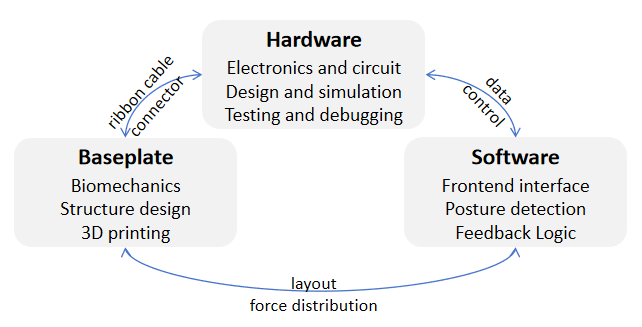
\includegraphics[width=0.75\textwidth]{Subsystem.png}
    \caption{Overview of the three main subsystems of HAPSeat—Hardware, Baseplate, and Software.}
    \label{fig:subsystems}
\end{figure}

% 硬件
\subsection{Hardware Development}
\subsubsection{Hardware Components}
% 本小节详细列出了系统使用的核心硬件原件
The hardware implementation relies on the following core components:

\begin{itemize}
    % 1. Arduino Uno 作为微控制器和系统电源，包含模拟和数字接口
    \item \textbf{Microcontroller:} An Arduino Uno serves as the central controller of the system and distributes power supplied through the laptop USB connection. It provides 5 analog inputs (with A4 and A5 dedicated to the I2C interface) and 13 digital I/O pins.
    
    % 2. 8个FSR，测量范围0-50kg，详见附录A.1
    \item \textbf{FSRs:} 8 FSRs are utilized to capture pressure distribution, with each sensor capable of measuring a weight range from 0 to 50 kg (\textit{Appendix \ref{app:fsr}}).
    
    % 3. 10个震动马达（5大5小），用于不同位置，详见附录A.2和A.3
    \item \textbf{Vibration Motors:} This configuration consists of 4 high-power motors (\textit{Appendix \ref{app:motor_high}}) and 5 low-power motors (\textit{Appendix \ref{app:motor_low}}) to meet the varying vibration intensity requirements at different anatomical contact points.
    
    % 4. CD74HC4067 16通道高速CMOS模拟多路复用器
    \item \textbf{Analog Multiplexer:} CD74HC4067, a High-Speed CMOS 16-Channel Analog Multiplexer (\textit{Appendix \ref{app:multiplexer}}).
    
    % 5. 16通道12位PWM驱动器
    \item \textbf{PWM Driver:} PCA9685, a 16-channel 12-bit PWM driver (\textit{Appendix \ref{app:PWM_controller}}).
    
    % 6. 8个10K分压电阻
    \item \textbf{Resistors:} 8 individual $10\text{k}\Omega$ voltage divider resistors are paired with the FSRs to facilitate accurate analog signal conversion.

    \end{itemize}
    
\subsubsection{Design Logic}
The FSRs are integrated using a straightforward voltage divider configuration. This setup converts the mechanical pressure-induced variable resistance into a measurable analog voltage signal. The output voltage ($V_{out}$) sampled by the analog multiplexer is determined by the following voltage divider equation:
\begin{equation}
    V_{out} = V_{cc} \times \frac{R_m}{R_{FSR} + R_m} = 5V \times \frac{10k\Omega}{R_{FSR} + 10k\Omega}
    \label{eq:voltage_divider}
\end{equation}
% Arduino Uno仅有5个模拟接口，无法直接读取8个FSR的数据
But the Arduino Uno has only 5 analog ports, which is insufficient to read 8 FSRs simultaneously. 
% 因此，系统使用模拟多路复用器，通过4个数字引脚高频切换来顺序读取传感器
Therefore, an analog multiplexer is used. It utilizes 4 digital pins to switch channels at high frequency, allowing one analog pin to sequentially sample all 8 sensors.

% 处理后，控制信号通过I2C传输到PWM驱动器
After software logic processing, control signals are sent to the PWM driver via the I2C interface. 
% PWM驱动器独立调节9个震动马达的强度
The PWM driver then independently modulates the vibration intensity of the 9 motors. 
% 电路原理图如下所示
The complete circuit schematic is shown in \textit{Figure \ref{fig:circuit_schematic}}.

% 插入原理图 test.pdf
\begin{figure}[htbp]
    \centering
    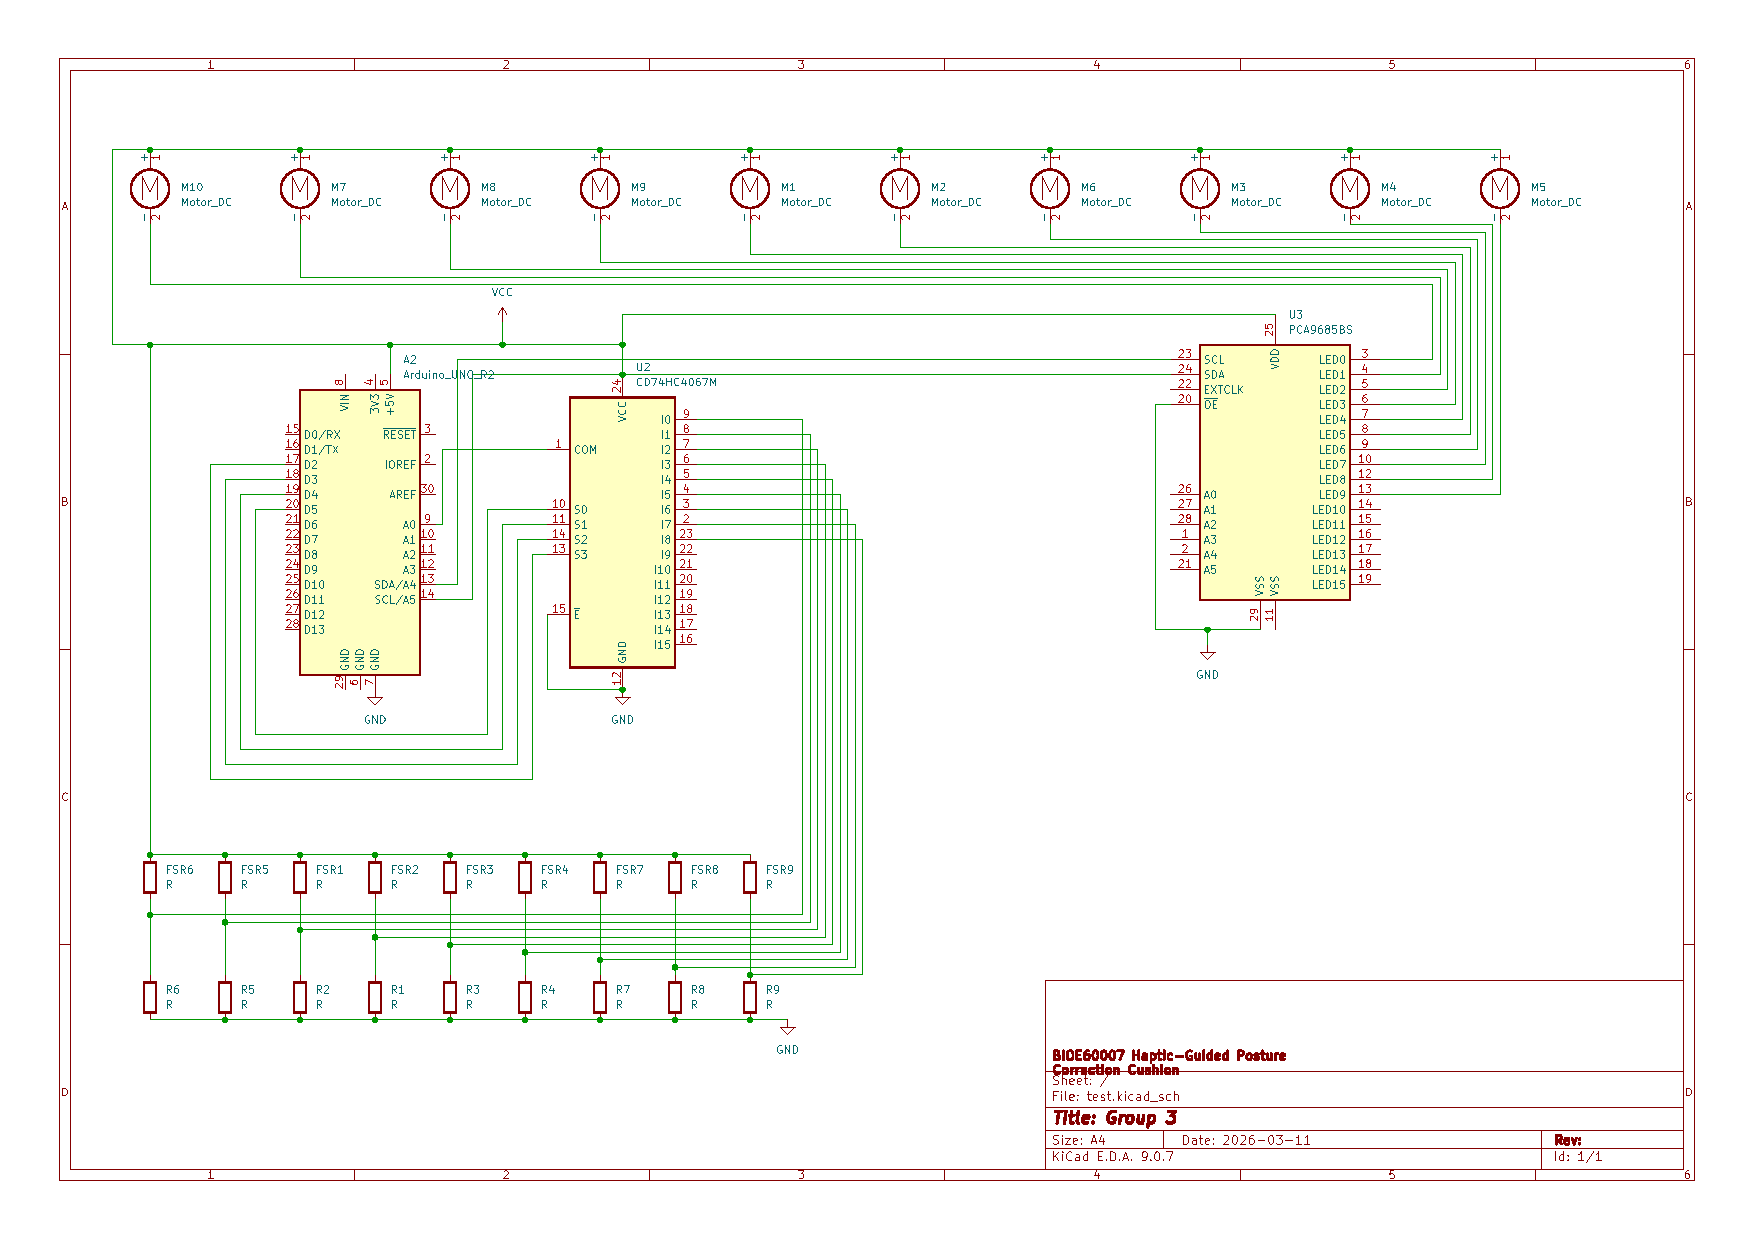
\includegraphics[width=\textwidth]{test.pdf}
    \caption{Circuit schematic connecting the microcontroller, multiplexer, FSRs, and PWM driver.}
    \label{fig:circuit_schematic}
\end{figure}
        
\subsubsection{Circuit Assembly}
% 主板尺寸控制在 9.4cm x 11.4cm 以内
The custom mainboard dimensions are constrained within $9.4\text{cm} \times 11.4\text{cm}$. A detachable Arduino Uno design facilitates debugging and minimizes the overall footprint. The circuit was independently routed and hand-soldered. 

% 增加外壳和绝缘层以防尘降噪和防止短路
Furthermore, a custom casing and insulation layer were implemented to reduce electrical noise and prevent dust-induced short circuits.


%%%%%%%%%%%%%% 【结构】 %%%%%%%%%%%%%%%%%
\subsection{Structural Development}

\begin{figure}[htbp]
    \centering
    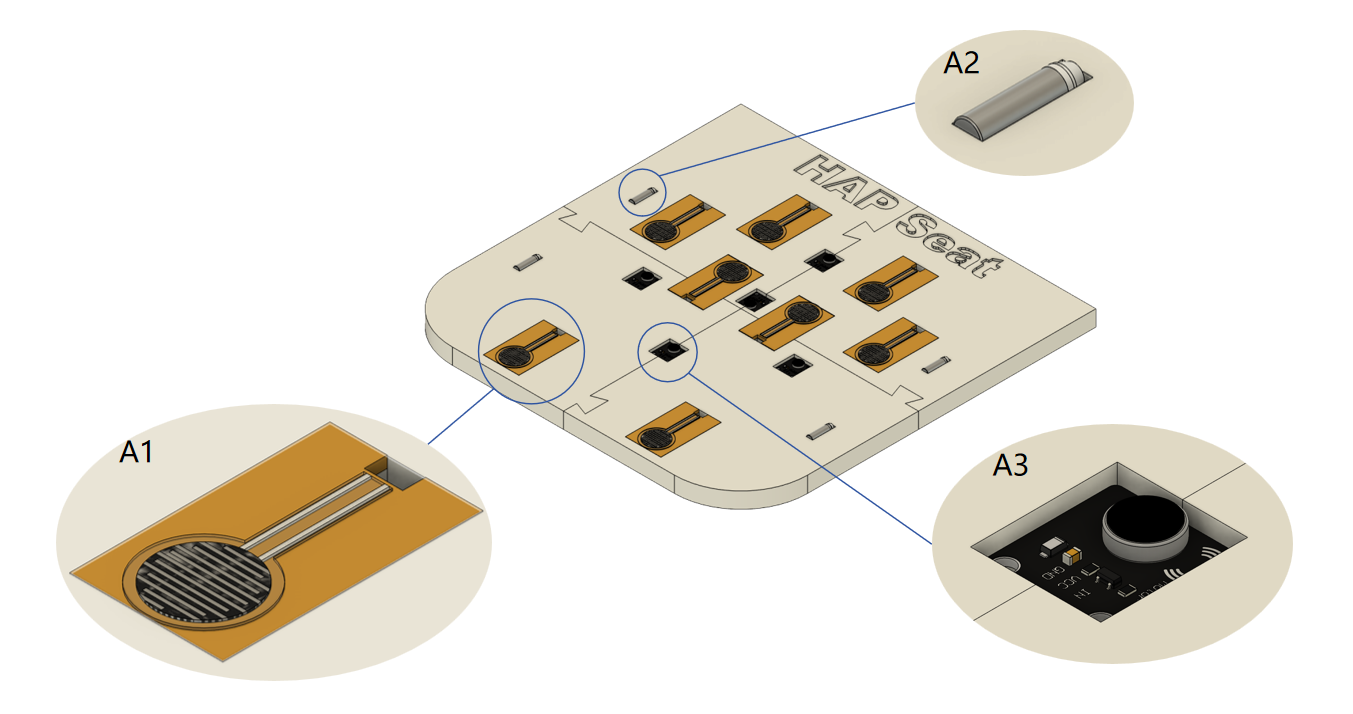
\includegraphics[width=\textwidth]{m1.png}
    \caption{Features on the upper side of the HAPSeat baseplate.}
    \label{fig:baseplate_top}
\end{figure}

\begin{figure}[htbp]
    \centering
    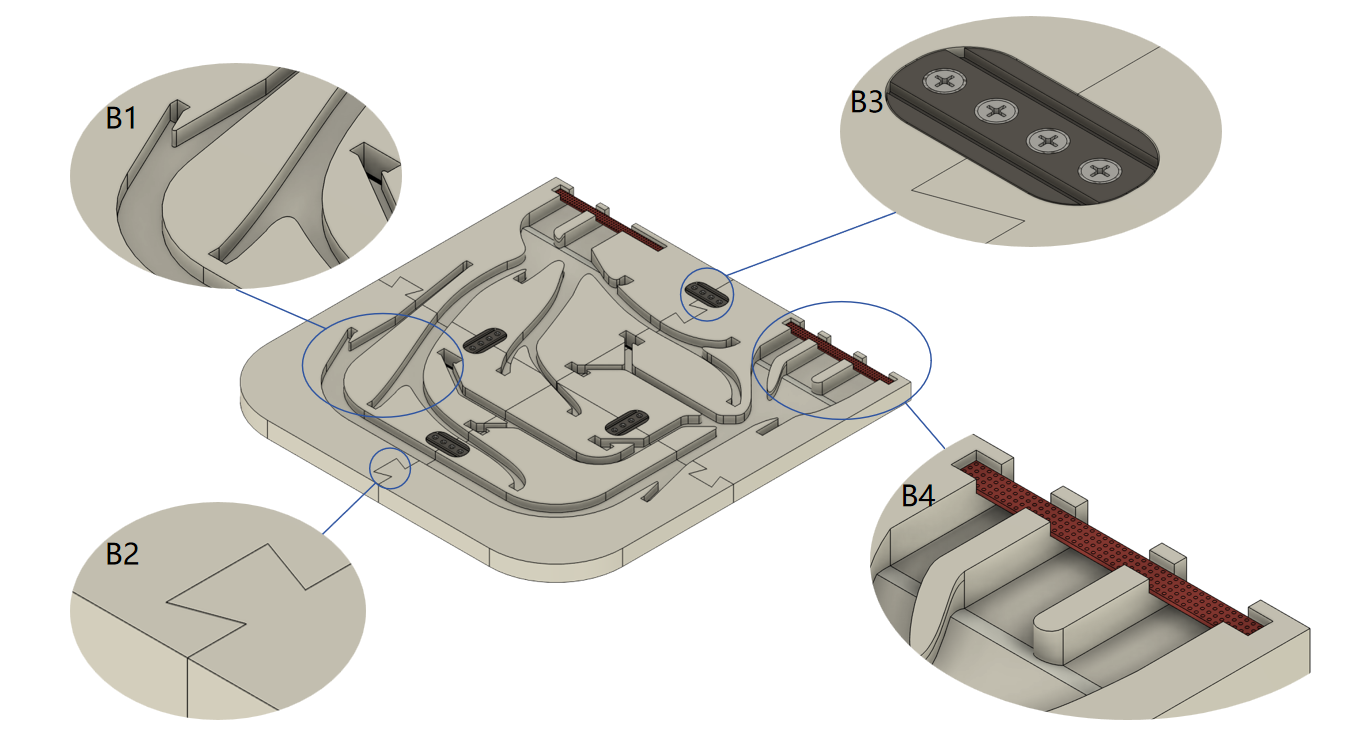
\includegraphics[width=\textwidth]{m2.png}
    \caption{Features on the underside of the HAPSeat baseplate.}
    \label{fig:baseplate_bottom}
\end{figure}

The hardware layout on the upside follows directly from the sensing and feedback principles above (shown in Figure 5). Since desirable sitting is characterised by balanced loading over the ischial regions, limited posterior collapse, and some thigh support, the sensing layer should prioritise these anatomical zones rather than sample the whole seat uniformly. The present prototype therefore places FSRs (A1) in three functional regions: a posterior region for detecting slumped or sacral sitting, a bilateral ischial region for monitoring the main load-bearing area, and an anterior thigh region for identifying forward load sharing. All  FSR modules were mounted on a 3 mm thick silicone pad (orange part), which helps with improving pressure-sensing performance. 
 
Meanwhile, the actuation layer is derived from the same principle. Because directional tactile cues can be produced by sparse actuator arrays \cite{Odesola2024SmartChairs, Israr2011TactileBrush, Dong2023DirectionalCues}, the current design concentrates stronger motors (A2) laterally around the buttock region, where feedback must remain perceivable through upholstery and soft tissue, while weaker motors (A3) are distributed along the seat midline and thigh-related regions to maintain directional continuity and reduce discomfort in more sensitive areas.

It should be noted that the prototype also includes an additional 3 mm silicone pad above the FSR layer, together with four foam cushions placed on top of it (two on each side), in order to further improve pressure sensing performance and user comfort. These layers are not illustrated in the figure, which is intended to highlight the structural design and component layout of the baseplate itself.



On the underside, the structure mainly serves reliability and mechanical stability (Figure 6). Features B1 and B4 together form the cable-routing system. B1 consists of dedicated routing channels that organise and secure the different wires, while B4 is the termination area where different wire groups are classified and soldered onto a perfboard. From this point, all wires are centrally connected to the controller circuit. This arrangement reduces the risk of poor electrical contact, simplifies troubleshooting, and improves overall system integration. Feature B2 shows that the 3D-printed baseplate segments are connected using dovetail interfaces, while Feature B3 is a joining strip fixed with four screws. Together, these two features reinforce the connection between adjacent baseplate sections and enhance the overall structural stability of the device.


%%%%%%%%%%%%%% 【软件】 %%%%%%%%%%%%%%%%%
\subsection{Software Development}

The software subsystem was implemented as a single self-contained HTML file in HTML, CSS, and JavaScript. Real-time data acquisition uses the Web Serial API to read the Arduino serial output at 9600 baud directly within the browser, avoiding server-side infrastructure.

Incoming serial frames---eight comma-separated FSR readings transmitted at approximately 30\,ms intervals---pass through three conditioning stages: channel remapping to anatomical zone positions, adaptive normalisation over a 48-frame rolling history with idle reset and a gain exponent of 0.58, and spatial spreading that yields a more coherent heatmap.

Posture classification compares the normalised FSR vector against six predefined posture prototypes using cosine similarity. Exponential moving average smoothing with a five-tick persistence requirement suppresses transient misclassifications, and confident predictions are mapped to predefined motor-routing patterns.

The front-end renders an SVG pressure heatmap, zone sparklines, a 30-second timeline, and an articulated silhouette driven by lightweight 2D affine transforms (Figure~\ref{fig:prototype}). Frame interpolation smooths the heatmap, while sidebar statistics update from each incoming packet to minimise perceived latency. A software-only demo mode enables full functional verification without connected hardware. Figure~\ref{fig:dashboard_ui} summarises the final interface.

\begin{figure}[H]
    \centering
    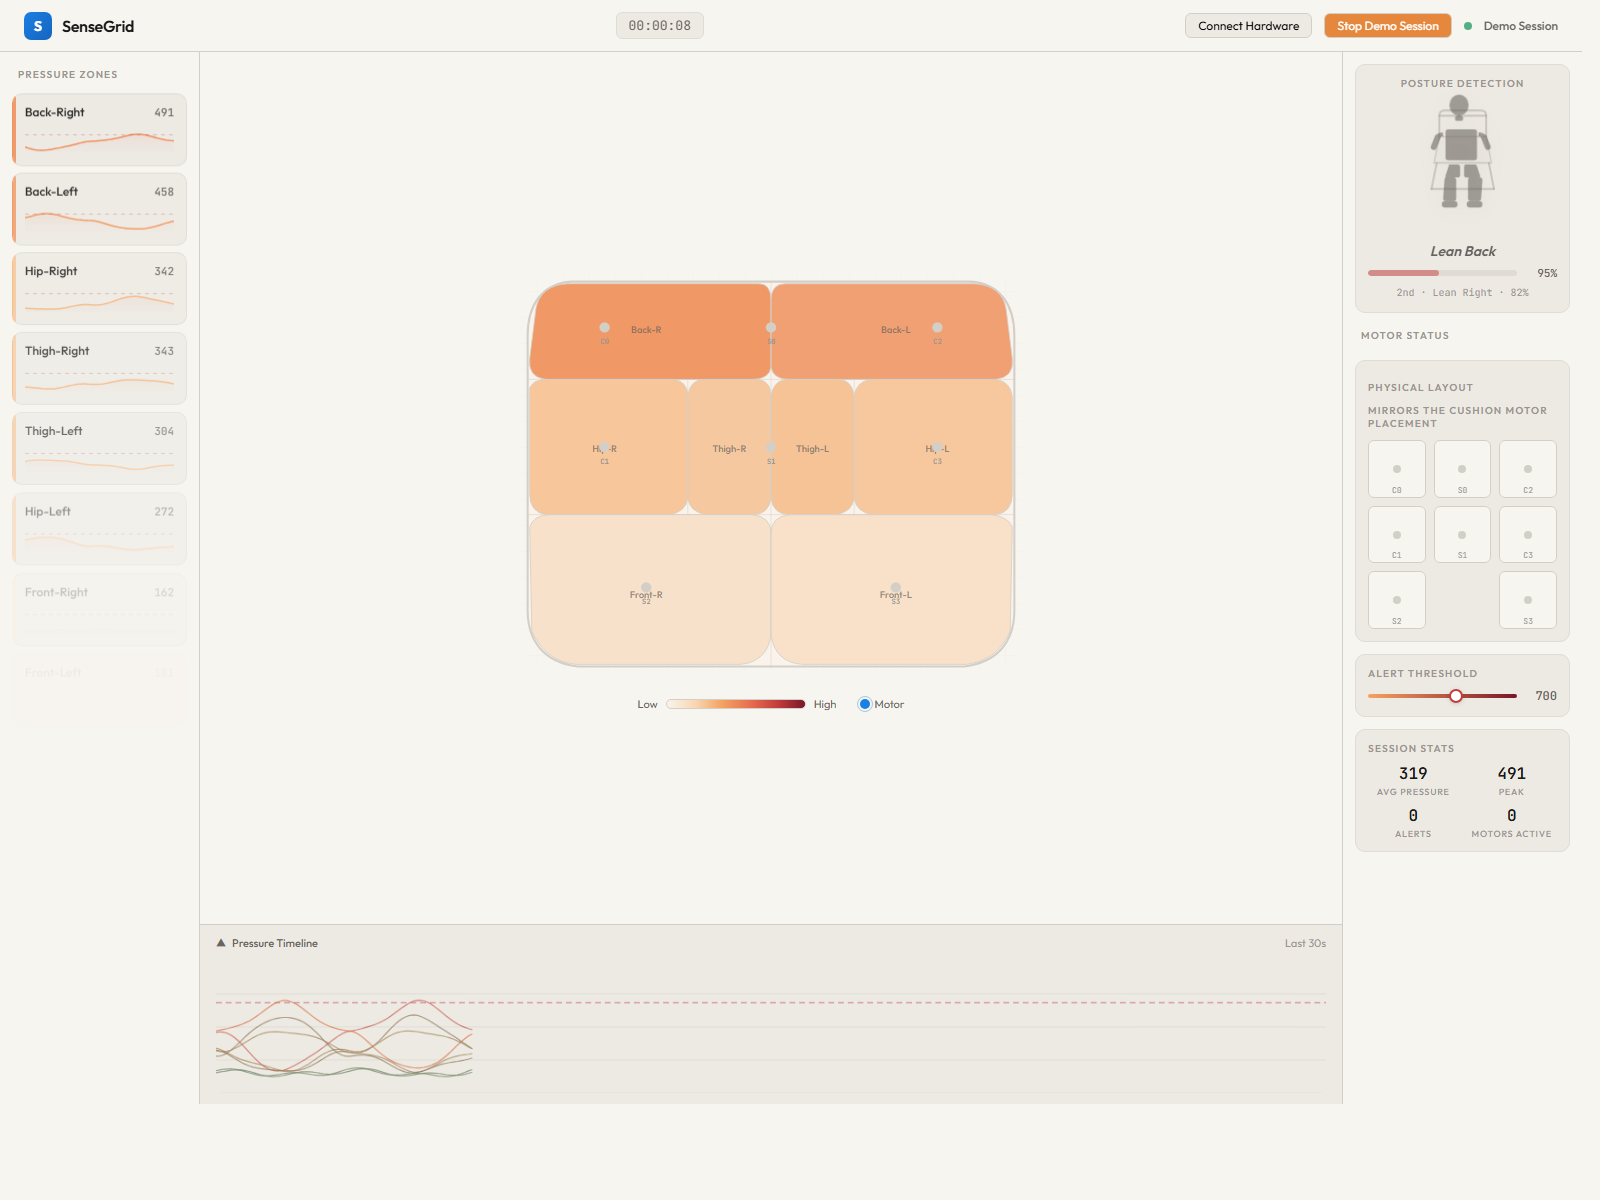
\includegraphics[width=0.84\textwidth]{dashboard_overview.png}

    \vspace{0.5em}

    \begin{minipage}[t]{0.28\textwidth}
        \centering
        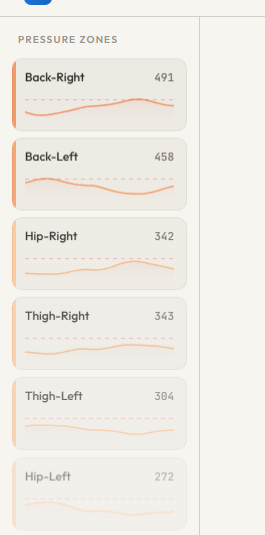
\includegraphics[width=\linewidth]{dashboard_zones.png}
    \end{minipage}
    \hfill
    \begin{minipage}[t]{0.28\textwidth}
        \centering
        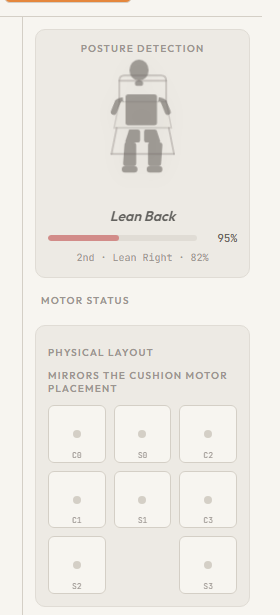
\includegraphics[width=\linewidth]{dashboard_posture.png}
    \end{minipage}
    \caption{Browser dashboard used during software testing and demonstration. The full interface is shown above, with zoomed views of the pressure-zone cards and sparklines (bottom left) and the posture and motor-status panels (bottom right).}
    \label{fig:dashboard_ui}
\end{figure}



%%%%%%%%%%%%%% 【评估】 %%%%%%%%%%%%%%%%%
% 5. 原型与评估---------------------------------
\section{Prototype and Evaluation}
\subsection{Prototype Implementation}
% BOM表
\subsubsection{BOM Table}

Table 1 summarises the key components used in the current HAPSeat prototype, including sensing, actuation, structural, wiring, and control elements.

\begin{table}[htbp]
    \centering
    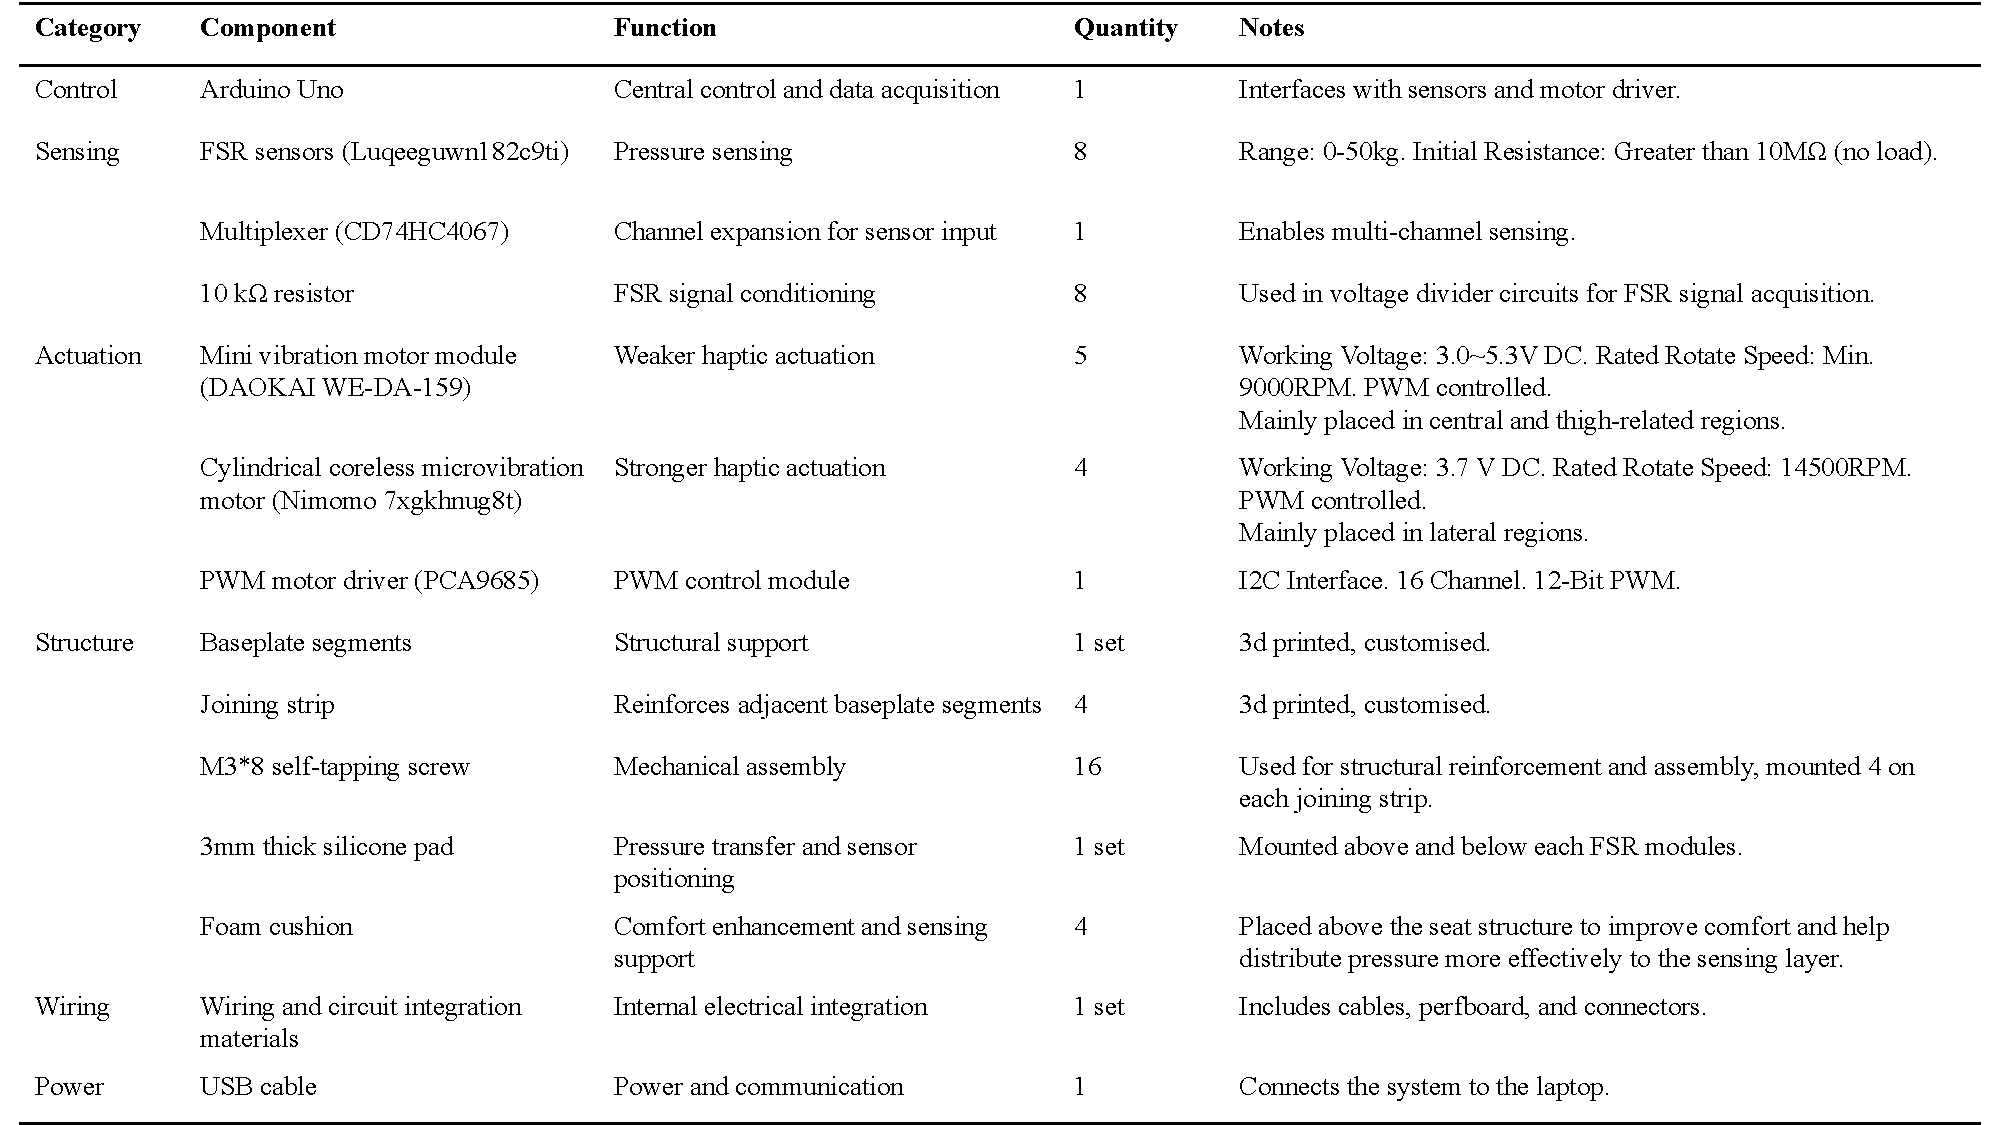
\includegraphics[width=1\textwidth]{BOM.pdf}
    \caption{Summary of the main components used in the current HAPSeat prototype.}
    \label{tab:BOM}
\end{table}

\subsubsection{System Workflow}
The entire prototype is powered and controlled through a laptop USB connection, following the signal and power pathway: laptop → Arduino → sensing and actuation subsystems.
FSR signals are sampled through the multiplexer, after which the software calculates pressure features. The trigger logic then determines whether asymmetry, slump, or prolonged static sitting is detected, and the PWM driver actuates the corresponding motor sequence.

\begin{figure}[htbp]
    \centering
    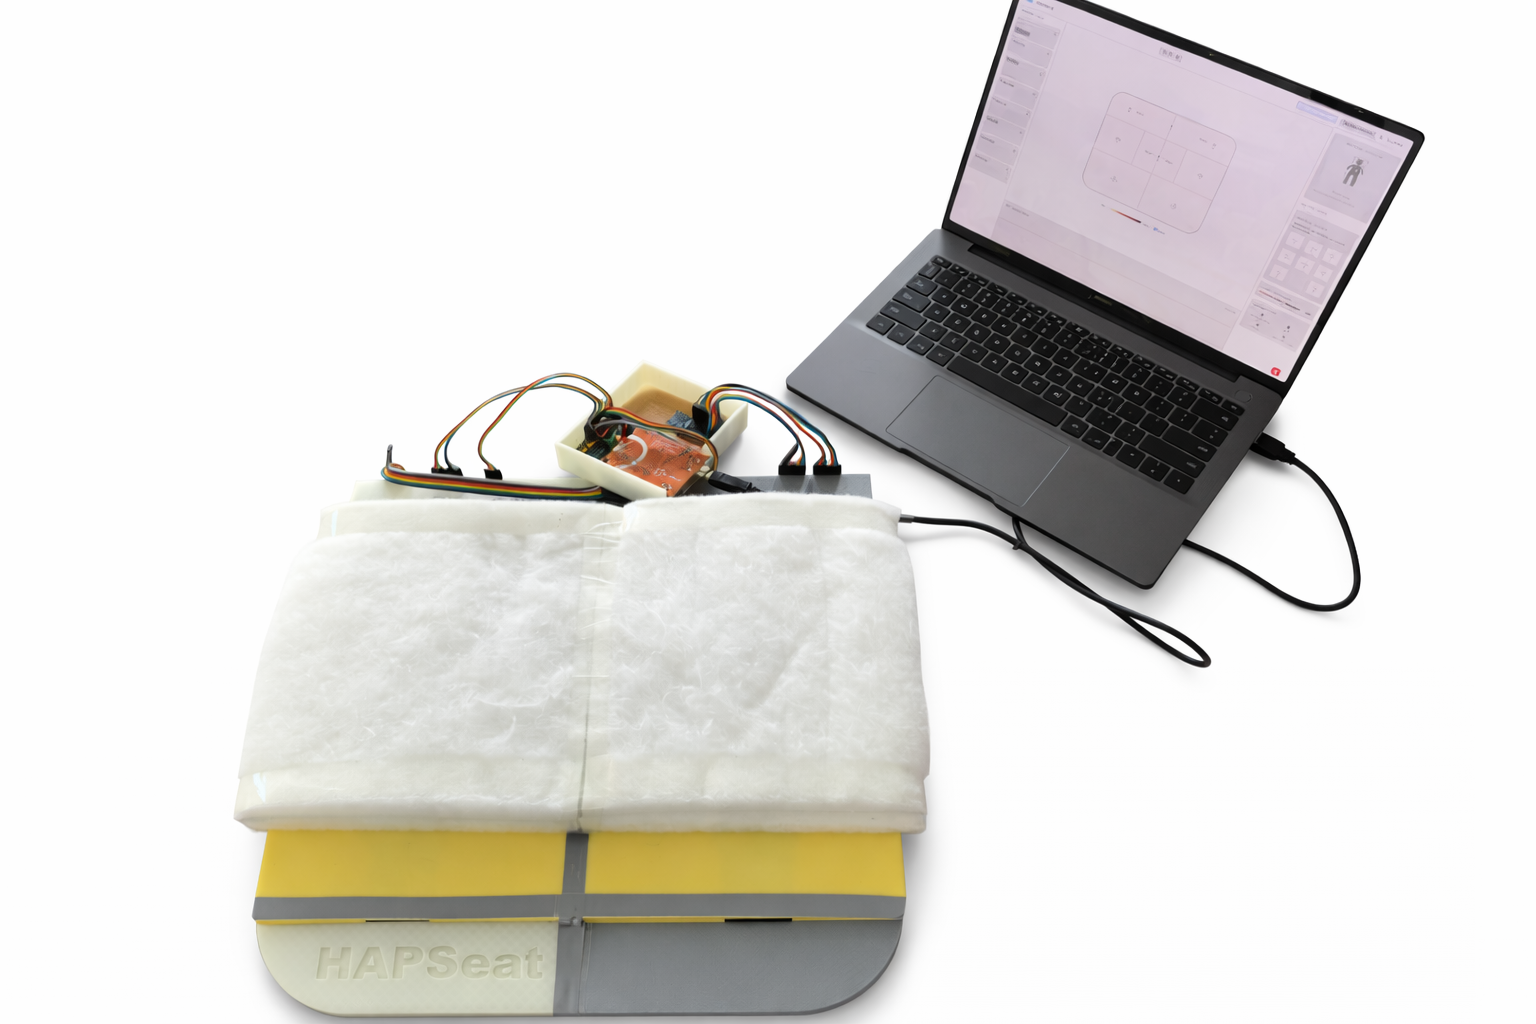
\includegraphics[width=0.75\textwidth]{prototype2.png}
    \caption{Current prototype and visual interface of HAPSeat.}
    \label{fig:prototype}
\end{figure}

\subsection{Evaluation Setup}

The current HAPSeat prototype was evaluated through a combination of functional testing and preliminary user-level testing. This evaluation was intended to assess whether the integrated system could reliably capture seat-pressure distribution, classify target posture conditions, and deliver interpretable feedback through both the visual and vibrotactile channels. At this stage, the evaluation should be regarded as a prototype-level assessment rather than a formal user study, as the testing was primarily conducted to verify system behaviour and identify major performance limitations.

Approximately 30 users participated in the prototype testing. Most were aged between 20 and 30 years, with a small number of users aged over 40. During testing, users were first asked to sit on HAPSeat and were guided to position themselves within the intended sensing region. Once seated correctly, the system response to different posture conditions, including forward leaning, backward leaning, left/right asymmetry, and leg crossing, was observed through both the heatmap interface and the corresponding vibration output.

\subsubsection{Functional Evaluation and User-Level Results}

The evaluation showed that the integrated sensing and visualisation pipeline functioned effectively. The front-end interface displayed a real-time pressure heatmap that was visually consistent with the actual seated pressure distribution, and this provided clear and intuitive visual feedback during testing. In practice, the heatmap was highly useful both for demonstrating system behaviour and for helping users understand how their posture affected seat loading.

Most users required some initial guidance in order to sit accurately within the effective sensing region. However, once correctly positioned, the system was able to detect major posture changes reliably. In particular, more than 90\% of users could be successfully identified when leaning forward, backward, left, or right. By contrast, detection of cross-legged sitting was less reliable. Although internal testing at an earlier stage suggested that cross-legged posture could sometimes be identified accurately, this behaviour was not sufficiently stable across users and test conditions.

The vibrotactile subsystem was generally successful in delivering perceivable feedback. Most users were able to feel the vibration cues, confirming that the actuation system functioned at a basic perceptual level. However, a substantial proportion of users could not clearly distinguish the intended direction of the vibration. As a result, the haptic output was more often experienced as a general posture reminder than as a precise directional guidance cue.

% 久坐模式的验证

%%%%%%%%%%%%%% 【总结】 %%%%%%%%%%%%%%%%%
% 6. 局限性与未来工作----------------------------
\section{Limitations and Future Work}
% 改进说法 改成guidance目前主要通过前端的视觉效果实现 而不是触觉反馈

The current limitations of HAPSeat can be grouped into three main areas: vibrotactile feedback effectiveness, sensing resolution, and practical usability. Among these, the most critical issues are the limited clarity of directional feedback and the insufficient sensitivity of the sensing system to subtle posture changes, as both directly affect the core functionality of the device. Future work should therefore prioritise improvements in actuation and sensing, including the exploration of alternative actuator types and the development of a higher-resolution custom sensing layer. Secondary priorities include improving seat compatibility and introducing user-specific calibration to support a wider range of body types and seating scenarios.

\clearpage
\begin{table}[p]
    \centering
    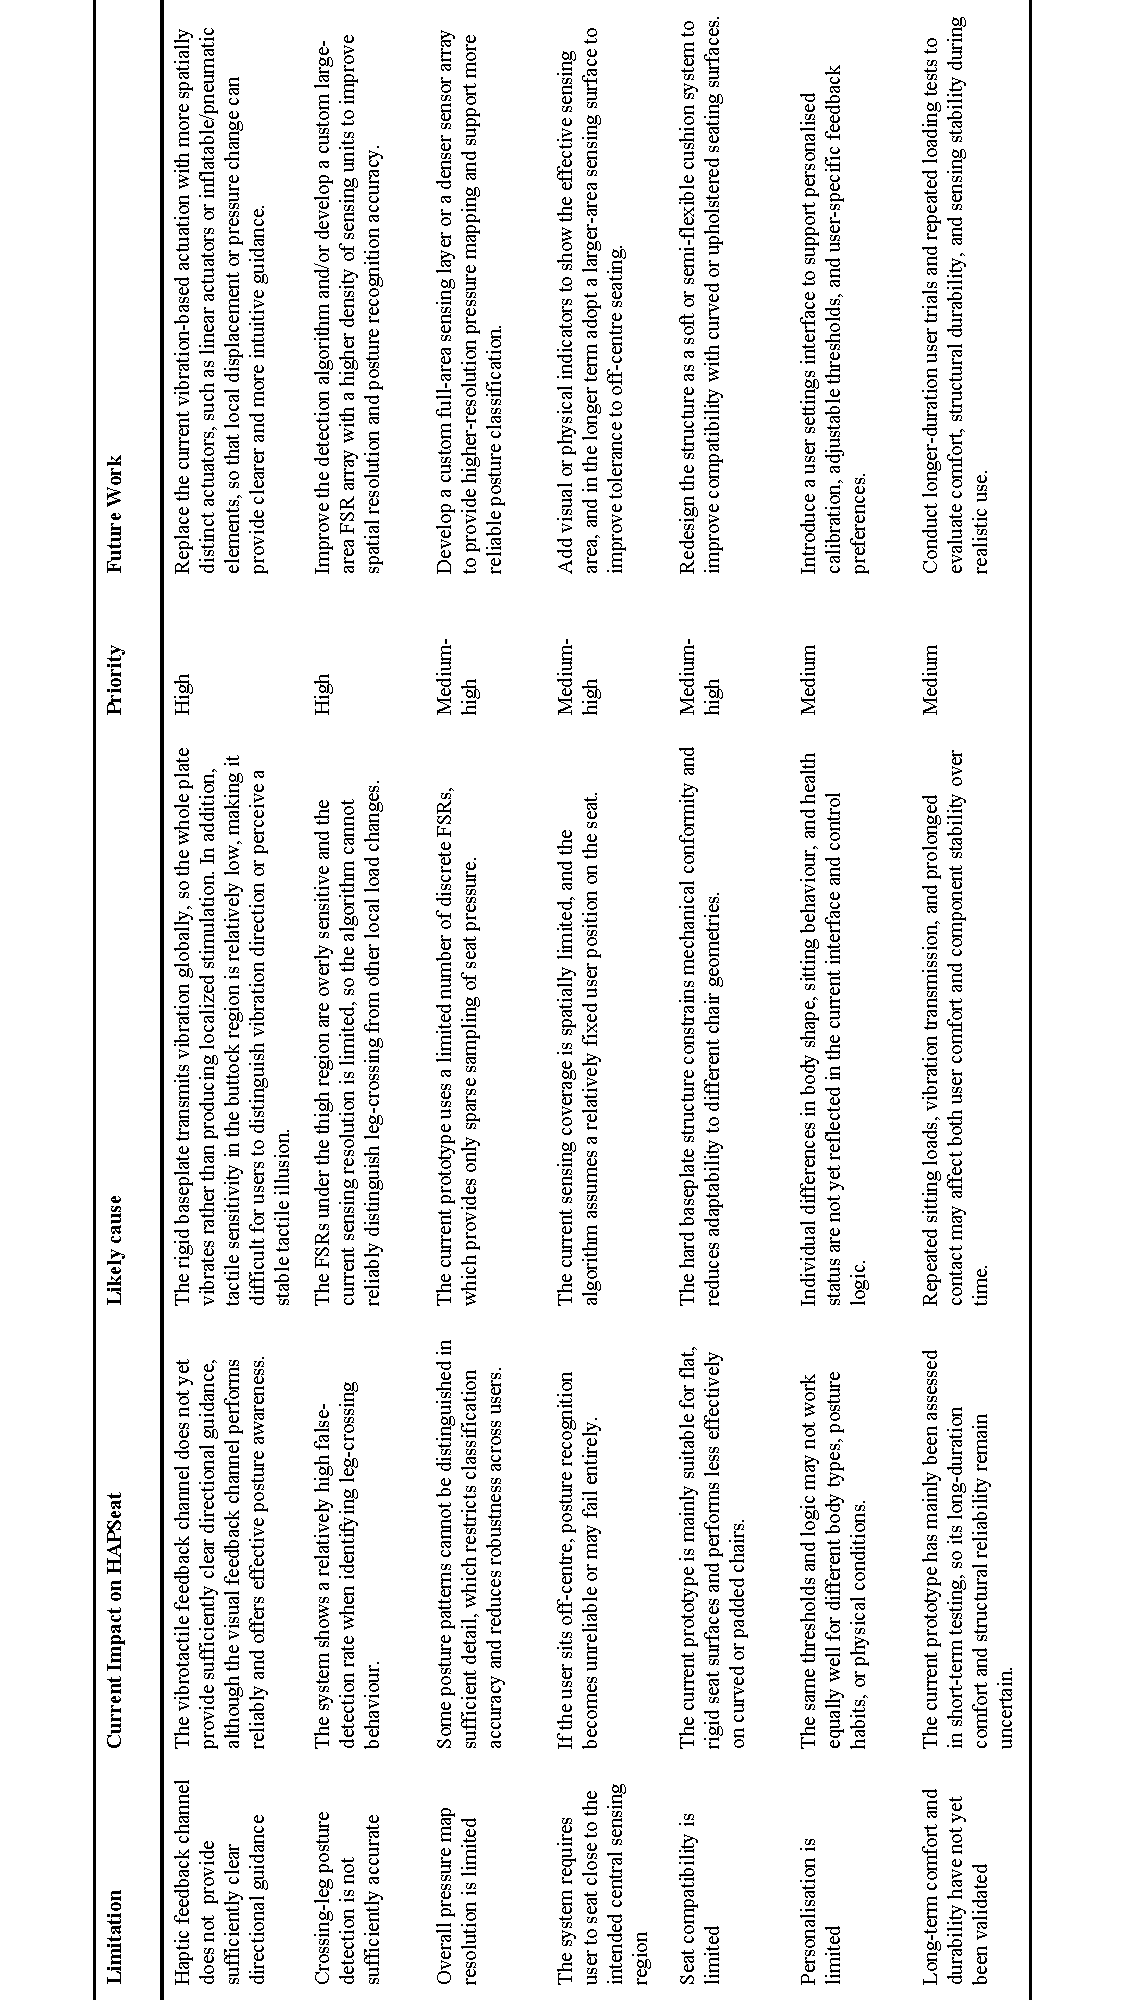
\includegraphics[width=0.85\textwidth]{Limitations.pdf}
    \caption{Summary of the main limitations of the current HAPSeat prototype, their impacts on system performance, priority levels, and corresponding directions for future work.}
    \label{tab:limitations}
\end{table}
\clearpage

\section{Conclusion}

This report presented HAPSeat, a multimodal posture support cushion integrating force-sensitive resistor sensing, browser-based visualisation, and vibrotactile feedback. The prototype showed that an eight-sensor array with adaptive conditioning and cosine-similarity posture classification can detect major postural deviations during seated work. The visual heatmap supported clear posture awareness, while vibrotactile cues remained perceivable but not yet directionally precise. Future work should prioritise higher-resolution sensing, alternative actuators, and user-adaptive calibration to move from monitoring toward directive haptic guidance.

%%%%%%%%%%%%%% 【文献】 %%%%%%%%%%%%%%%%%
% 参考文献-------------------------------------
\newpage
\printbibliography


% 附录-----------------------------------------
\newpage
\appendix

% 原件参数
\section{Components Parameters:}
\label{app:detailed_bom}

The appendix tables below summarise the final prototype configuration described in the report together with the key interface specifications of the core electronic components.

% 附录 A.1：FSR传感器详细参数
%%%%%%%%%%%%%% 【尺寸】 %%%%%%%%%%%%%%%%%
\subsection{FSR Sensor Specifications}
\label{app:fsr}

\begin{table}[H]
    \centering
    \footnotesize
    \begin{tabular}{p{0.34\textwidth} p{0.58\textwidth}}
        \toprule
        \textbf{Parameter} & \textbf{Specification} \\
        \midrule
        Sensor type & Force-sensitive resistor (FSR) pressure sensor \\
        Quantity in prototype & 8 \\
        Nominal measurement range & 0--50 kg per sensor \\
        Electrical behaviour & Variable resistance that decreases with increasing applied load \\
        Readout circuit & 5 V voltage-divider interface with an individual $10\,\text{k}\Omega$ resistor per sensor \\
        Sampling path & Sequentially sampled through the CD74HC4067 multiplexer into the Arduino Uno analog input \\
        Placement strategy & Distributed across posterior, bilateral ischial, and anterior thigh regions of the seat \\
        Functional role & Supports symmetry detection, anterior load sharing assessment, posterior collapse detection, and temporal variation monitoring \\
        \bottomrule
    \end{tabular}
\end{table}

% 附录 A.2：大功率震动马达参数
%%%%%%%%%%%%%% 【尺寸】 %%%%%%%%%%%%%%%%%
\subsection{High-Power Vibration Motors}
\label{app:motor_high}

\begin{table}[H]
    \centering
    \footnotesize
    \begin{tabular}{p{0.34\textwidth} p{0.58\textwidth}}
        \toprule
        \textbf{Parameter} & \textbf{Specification} \\
        \midrule
        Motor class & High-power vibration motors used for stronger haptic cues \\
        Quantity in prototype & 4 \\
        Placement strategy & Concentrated laterally around the buttock region \\
        Drive method & Individually PWM-controlled through the PCA9685 driver \\
        Design rationale & Higher output is required where vibration must remain perceivable through upholstery and soft tissue \\
        Primary corrective role & Provides the dominant lateral and posterior corrective cues in the guidance sequences \\
        Integration with control logic & Activated by the software trigger logic when asymmetric or slumped pressure patterns are detected \\
        \bottomrule
    \end{tabular}
\end{table}

% 附录 A.3：小功率震动马达参数
%%%%%%%%%%%%%% 【尺寸】 %%%%%%%%%%%%%%%%%
\subsection{Low-Power Vibration Motors}
\label{app:motor_low}

\begin{table}[H]
    \centering
    \footnotesize
    \begin{tabular}{p{0.34\textwidth} p{0.58\textwidth}}
        \toprule
        \textbf{Parameter} & \textbf{Specification} \\
        \midrule
        Motor class & Low-power vibration motors used for continuity and comfort-sensitive cueing \\
        Quantity in prototype & 5 \\
        Placement strategy & Distributed along the seat midline and thigh-related regions \\
        Drive method & Individually PWM-controlled through the PCA9685 driver \\
        Design rationale & Maintains directional continuity while reducing discomfort at more sensitive contact points \\
        Primary corrective role & Supports ripple-style guidance, movement encouragement, and completion of multi-motor cue sequences \\
        Integration with control logic & Coordinated with the high-power motors to form the full distributed haptic guidance array \\
        \bottomrule
    \end{tabular}
\end{table}

% 附录 A.4：Multiplexer 参数
\subsection{Analog Multiplexer (CD74HC4067)}
\label{app:multiplexer}

\begin{table}[H]
    \centering
    \footnotesize
    \begin{tabular}{p{0.34\textwidth} p{0.58\textwidth}}
        \toprule
        \textbf{Parameter} & \textbf{Specification} \\
        \midrule
        Device & CD74HC4067 \\
        Function & 16-channel analog multiplexer/demultiplexer \\
        Supply voltage range & 2 V to 6 V \\
        Channel selection & 4 digital select lines with break-before-make switching \\
        Typical on-state resistance & 60 $\Omega$ at 5 V \\
        Prototype usage & 8 FSR channels read through channels 8--15 into one Arduino analog input \\
        Signal role in HAPSeat & Expands the Arduino Uno analog input capacity so all seat-pressure sensors can be sampled within the same acquisition cycle \\
        Operating temperature range & $-55\,^{\circ}\text{C}$ to $125\,^{\circ}\text{C}$ \\
        \bottomrule
    \end{tabular}
\end{table}

% 附录 A.5：PWM controller 参数
\subsection{PWM Driver (PCA9685)}
\label{app:PWM_controller}

\begin{table}[H]
    \centering
    \footnotesize
    \begin{tabular}{p{0.34\textwidth} p{0.58\textwidth}}
        \toprule
        \textbf{Parameter} & \textbf{Specification} \\
        \midrule
        Device & PCA9685 \\
        Function & 16-channel, 12-bit PWM controller \\
        Interface & Fast-mode Plus I$^2$C bus (up to 1 MHz) \\
        Supply voltage range & 2.3 V to 5.5 V \\
        PWM resolution & 4096 steps \\
        Programmable PWM frequency & Approximately 24 Hz to 1526 Hz \\
        Prototype configuration & Operated at 1000 Hz to drive the vibration motors \\
        Output capability & Totem-pole outputs with 25 mA sink and 10 mA source capability at 5 V \\
        Signal role in HAPSeat & Provides independent intensity control for the distributed vibration motor array \\
        Operating temperature range & $-40\,^{\circ}\text{C}$ to $85\,^{\circ}\text{C}$ \\
        \bottomrule
    \end{tabular}
\end{table}



\end{document}
